% LaTeX-mal for labrapporter i FY1001 Mekanisk fysikk, NTNU
% Jonas Tjemsland og Rolf Jonas Persson september 2021
% Basert på LaTeX-mal for labrapporter i FY1001, v.01.11.2011, og tidligere labhefter.

\documentclass[5p]{elsarticle}
% I klammeparantesen kan vi definere noen parametere som er spesifikt for hver klasse.
% For eksempel gir "5p" 2 kolonner per side, og 1p gir 1 kolonne per side. Dette er spesifikt for elsarticle.

% Vi laster inn en del pakker i starten av dokumentet som inneholder kommandoer og miløer vi vil få bruk for.
\usepackage[utf8]{inputenc}                   % Mulighet til å skrive utf8-symboler
\usepackage[norsk]{babel}				      % Tilpasning til norsk
\usepackage{graphicx}       				  % For å inkludere figurer
\usepackage{amsmath,amssymb} 				  % Ekstra matematikkfunksjoner
\usepackage[font=small,labelfont=bf]{caption} % For justering av figurtekst og tabelltekst
\usepackage{hyperref}                         % For å skrive klikkbare linker
\usepackage{minted}

% Vi kan også definere egne funksjoner
\newcommand{\enhet}[1]{~\mathrm{#1}}  % Kommando for å enklere typesette enheter
\newcommand{\dd}[2]{\frac{\mathrm{d}{#1}}{\mathrm{d}{#2}}} % i stedet for \frac{d}{d} 

% Gjør noen fornorskinger (vanligvis holder et med pakken "babel", men Elsarticle ødelegger)
% Endrer fra "Preprint submitted to" til "Preprint forelagt"
\usepackage{etoolbox}
\makeatletter\patchcmd{\ps@pprintTitle}{Preprint submitted to}{Preprint forelagt}{}{}\makeatother
% Abstract -> Sammendrag
\abstracttitle{Sammendrag} % Spesifikt for elsarticle

% Her skriver man tittel og forfatterinformasjon
\title{Dempet rullebevegelse i bunnen av sirkelformet bane}
\author[fysikk]{T. C. Djupvik}
\author[fysikk]{O. F. Jakobsen}
\address[fysikk]{Institutt for fysikk, Norges Teknisk-Naturvitenskapelige Universitet, N-7491 Trondheim, Norway.}
\journal{Labveileder} % Leveres til labveileder

%%%%%%%%%%%%%%%%%%%%%%%%%%%%%%%%%%%%%%%%%%%%%%%%%%%%%%%%%%%%%%%%%%%%%%%%%
\begin{document}

\begin{abstract}

\textit{Her skriver du et sammendrag av rapporten. Sammendraget skal være veldig kort
men må inneholde svaret på tre spørsmål: 1. Hva gjorde du (hva målte du)? 2. Hvordan 
gjorde du det (hvilken metode)? 3. Hva fant du (resultat)?}
\end{abstract}

\maketitle % Denne kommanoden skriver ut dokumentinformasjonen, overskrift og sammendrag.

%%%%%%%%%%%%%%%%%%%%%%%%%%%%%%%%%%%%%%%%%%%%%%%%%%%%%%%%%%%%%%%%%%%%%%%%%
\section{Innledning}
I dette prosjektet undersøkes det hvilke effekter som bremser opp bevegelsen 
til en sylinder som ruller rent i bunnen av en sirkelformet bane. Det kommer ikke til å 
bli tatt hensyn til sluring, men både luft- og rullemotstand kommer til å bli tatt med i modellen.
Ved å sammenligne de eksperimentelle målingene med de numeriske og analytiske løsningene av 
ligningen som beskriver systemet ønsker vi å anslå verdier for de ulike dempeeffektene. 
I tillegg vil det bli diskutert hvordan de ulike bremsekreftene varierer alt etter hvor sylinderen 
er i banen.
\par
Videre vil diskusjonen sammenligne måleseriene av ulike sylindre, og ...

%%%%%%%%%%%%%%%%%%%%%%%%%%%%%%%%%%%%%%%%%%%%%%%%%%%%%%%%%%%%%%%%%%%%%%%%%
\section{Teori}

For å beskrive bevegelsen til sylinderen kan man bruke Newtons andre lov i tangentiell retning.
Man kan da finne et uttrykk for \(\ddot{\phi}\) gitt ved \(\dot{\phi}\) og \(\phi\). 
Denne differensialligningen inneholder også de tre dempekreftene \(f_S\), \(f_D\) og \(f_R\), 
som henholdsvis inneholder diverse dempekrefter, luftmotstand og rullefriksjon.

\begin{align}
	\vec{f_S} & = -\tilde{\delta} \vec{v} 			\\
	\vec{f_D} & = -\tilde{\beta}|\vec{v}|^2\hat{v}  \\
	\vec{f_R} & = -|\vec{f_R}|\hat{v}				
\end{align}

Her er \(\tilde{\delta}\) \textit{dempingskonstanten},\(\tilde{\beta}\) \textit{dragkoeffisienten}.
Det kan vises at \(F_R\) kan uttrykkes ved

\begin{equation}
	|f_R|\text{sgn}\dot{\phi} =
	m\left[
		cl\ddot{\phi}+\frac{d}{r}
		\left(l\dot{\phi}^2 + g\cos\phi\right)
		\text{sgn }\dot{\phi}
	\right]
\end{equation}

Ved å bruke Newtons andre lov på den rullende sylinderen 
og bruke ligningen for \(f_R\) kommer man frem til følgende uttrykk:

\begin{equation}
	\begin{split}
		\label{ODE}	
		\ddot{\phi} = 	
		&- \omega_0^2\sin\phi - 2\delta\dot{\phi}	\\
		&- \frac{\pi\phi_R}{2\omega_0}
		\left(\omega_0^2\cos\phi + \gamma\dot{\phi}^2\right) \text{sgn } \dot{\phi} \\
		&- \beta \frac{3\pi}{4\omega_0}\dot{\phi}^2\text{sgn }\dot{\phi} 
	\end{split}
\end{equation}

Her er størrelsene \(\delta\), \(\beta\) og \(\phi_R\) skalerte versjoner av 
\(\tilde{\delta}\), \(\tilde{\beta}\) og \(d\), der \(d\) er armen til normalkraften (se figur \ref{Fig System})

Å løse differensialligninger eksakt vil i de fleste tilfeller være svært vanskelig eller umulig.
Likevel kan man løse \eqref{ODE} i noen grensetilfeller. Ved å bare se på \(\phi << 1\) vil man kunne
bruke approksimasjonene 
\(\sin(\phi) = \phi + \mathcal{O}(\phi^3) \approx \phi\) og 
\(\cos(\phi) = 1 + \mathcal{O}(x^2) \approx 1\).
I tillegg vil man kunne finne eksakte løsninger ved å sette to av \(\delta\), \(\beta\) og \(\phi_R\) lik 0.
\par
Selv om man i noen tilfeller kan finne analytiske løsninger 
vil det i mange tilfeller være mer hensiktsmessig å løse differensialligningen numerisk.
\eqref{ODE} er en ordinær differensialligning av andre orden. 
Denne kan skrives som to koblede førsteordens ordinære differensialligninger ved å innføre \(u = \dot{\phi}\):

\begin{subequations}
	\begin{align}
		\dd{\phi}{t} & = u \\
		\dd{u}{t}    & = f(\phi, u) \\
	\end{align}
\end{subequations}

Dette ligningssettet kan løses diskret ved bruk av Eulers metode. 
Man løser da

\begin{subequations}
	\begin{align}
		\label{Newton}
		\phi_{i+1} & = \phi_i + u_i \Delta{t} \\
		u_{i+1}    & = u_i + f(\phi_i, u_i) \Delta {t} 
	\end{align}
	for en valgt \(\Delta t\) og med startverdiene \(\phi_0\) og \(u_0 = \dot{\phi_0}\)
\end{subequations}

Da Eulers metode ofte fører til systematisk avvik, er det bedre å bruke Crank-Nicholson-metoden. (ref her?)

\begin{figure}[] 
% Alternativene inne i klammene angir hvilke av følgende plasseringer du vil tillate:
% h = here, t = top, b = bottom, p = separat, ! = forsøk å overstyre preferansene til LaTeX.
% (Preferansene til LaTeX gjør noen ganger at figurer ikke havner der du selv mener de passer best...).
  \begin{center}
      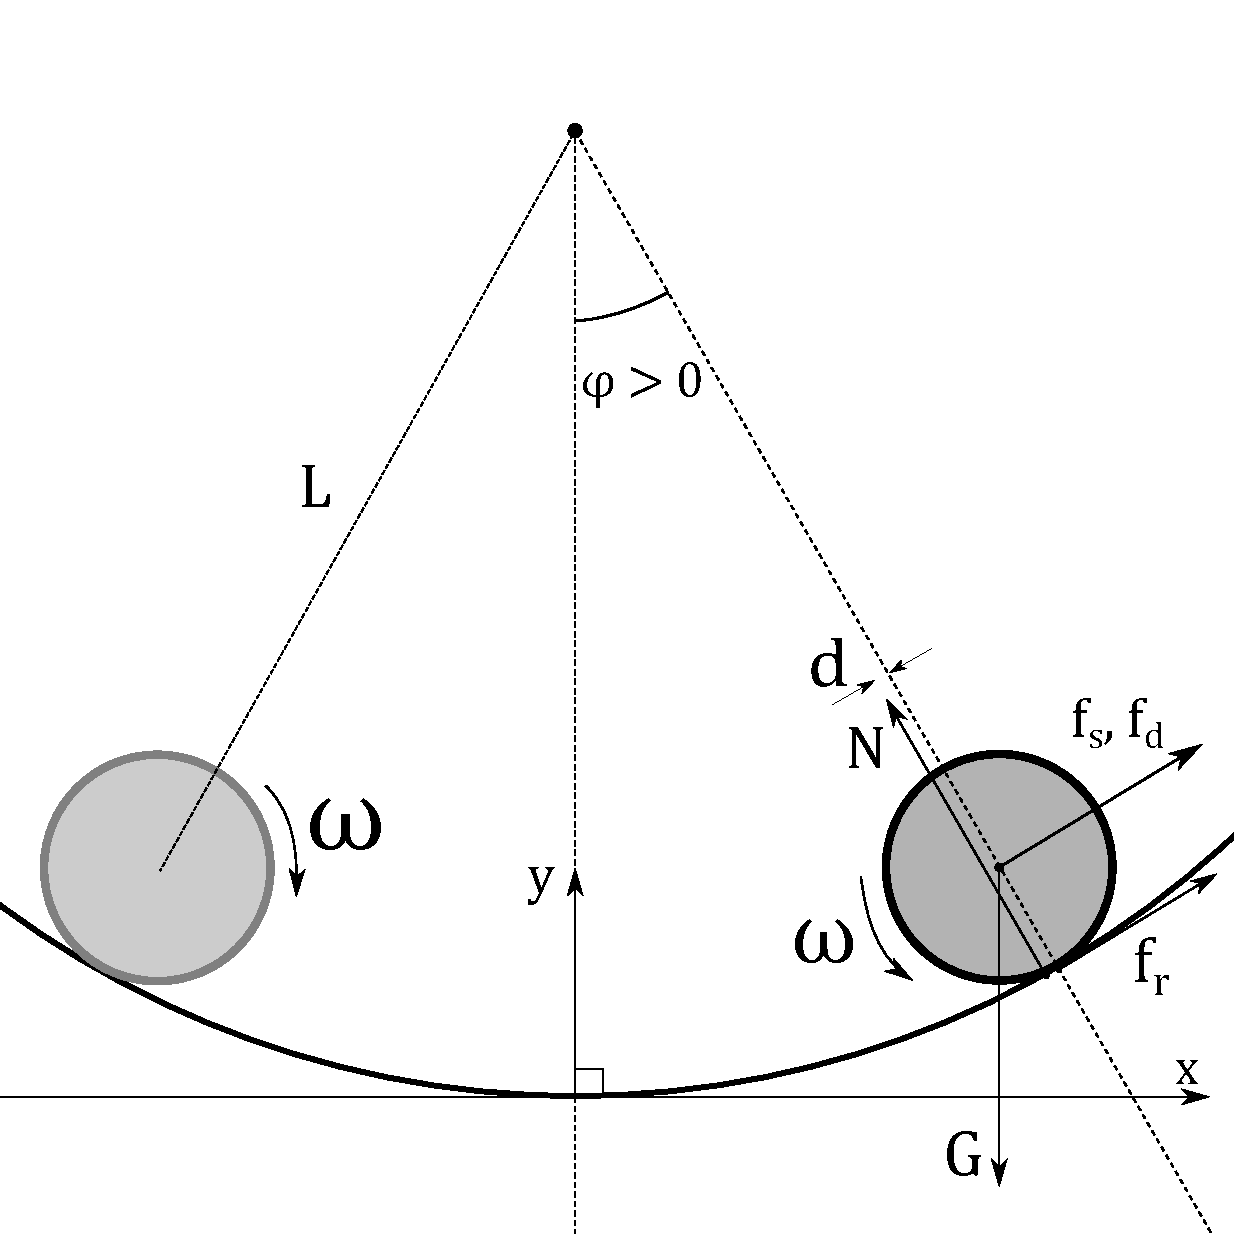
\includegraphics[width=0.4\textwidth]{drawing2}  % Putter inn fila pendel.pdf
%   Hvis du angir bare enten width eller height, beholdes originalfigurens proporsjoner. (Dette anbefales.)
% 	Her har vi brukt width=0.3\textwidth for å angi figurbredde som en andel av den delen av arkbredden som inneholder tekst.
  \end{center}
  \caption{Skisse av system.}
  \label{Fig System} % Som med ligningen, er dette navnet vi refererer til.
\end{figure}

%%%%%%%%%%%%%%%%%%%%%%%%%%%%%%%%%%%%%%%%%%%%%%%%%%%%%%%%%%%%%%%%%%%%%%%%%
\section{Metode}
\noindent\textbf{Utstyr}:
\begin{itemize}
	\item Kvartsirkel i stål (\(R = 46 \enhet{cm}\))
	\item Tre ulike sylindre:
	\\ Sylinder 1 - massiv plast
	\\ Sylinder 2 - liten metall solid 
	\\ Sylinder 3 - liten metall hul
	\item Kamera med tripod Panasonic DMC-FZ-200
	\item Videoanalyseprogrammet Tracker
	\item Meterstav, skyvelær, vekt
\end{itemize}

I dette forsøket brukes Tracker til å samle inn måleserier. 
Først gjøres det et testopptak for å passe på at lys- og fokusinnstillinger på kameraet er gode nok for videre analyse.
Deretter blir sylinderen satt i sirkelbanen. (Se figur \ref{Fig Oppsett})
Ved å bruke autotracker-funksjonen i Tracker får man deretter ut måleserier med posisjonsdata.
Videre analyser \dots 
(legg inn tweaking + scipy) 

\begin{figure}[] 
	\begin{center}
		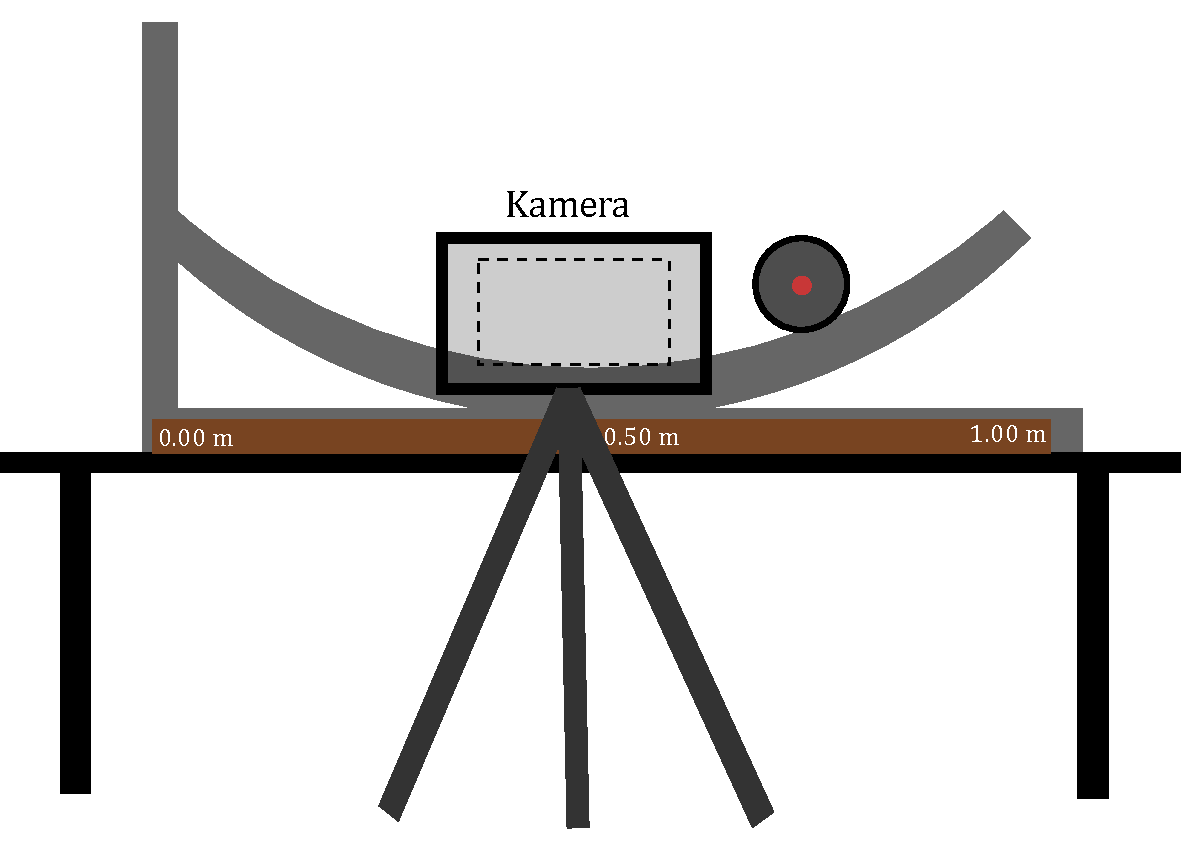
\includegraphics[width=0.4\textwidth]{skisse}
	\end{center}
	\caption{Skisse av oppsett.}
	\label{Fig Oppsett} % Som med ligningen, er dette navnet vi refererer til.
\end{figure}

%%%%%%%%%%%%%%%%%%%%%%%%%%%%%%%%%%%%%%%%%%%%%%%%%%%%%%%%%%%%%%%%%%%%%%%%%
\section{Resultat}

Ved implementering av Eulers metode får man: (plot Euler)
Ved å variere \(\Delta t\) får vi følgende resultater.
Likeledes gir CN-metoden følgende: (plot)
Ved å variere \(\Delta t\) får vi følgende resultater.
(plotting)

Eksperimentering av ulike verdier for \(phi_R\), \(\delta\) og \(\beta\)
Må vurdere hvor mange plots som er hensiktsmessig. Kanskje bare ta med to måleserier?

\begin{table}[htb]
	\begin{center}
		\caption{Målinger av de ulike sylindrene.}
		\label{MinLilleTabell}	% Merkelappen vi vil referere til.
		% \vspace{0.5cm}	% Litt ekstra plass for å få det til å se penere ut.
		\begin{tabular}{lrrr} 		% Tre venstrejusterte kolonner (l = left, c = center, r = right).
			\hline 								% Horisontal linje.
		    Sylinder &  masse  & indre diameter & ytre diameter \\ % Merk symboler i kursiv, (men det er fordi de er symboler, ikke fordi de er kolonneoverskrifter!)
			&  (g)    &   (mm)   &  (mm)    \\ % mens enheter ikke er det.
			\hline												
			1   &  442 \(\pm\)0.5 & 	  & 73.5\(\pm\)0.1 \\ % Stor plast solid
			2   &  1097\(\pm\)0.5 & 	  & 44.5\(\pm\)0.1 \\ % Liten metall solid
			3   &  255 \(\pm\)0.5 & 42.4\(\pm\)0.1 & 36.5\(\pm\)0.1 \\ % Liten metall hul
			% Usikkerhet &  \(\pm\)0.5 & \(\pm\) 0.1 & \(\pm\) 0.1 \\
			\hline
		\end{tabular}
	\end{center}
\end{table}

%%%%%%%%%%%%%%%%%%%%%%%%%%%%%%%%%%%%%%%%%%%%%%%%%%%%%%%%%%%%%%%%%%%%%%%%%

\section{Diskusjon}
\textit{Her er det konklusjonen av resultatene dine som skal diskuteres, og
for å kunne diskutere dette må du sette dem inn i en større
sammenheng. Dette gjør du ved å relatere resultatene dine til
tidligere utførte undersøkelser på samme område, og ved å forutsi de
konsekvenser som resultatene av din undersøkelse medfører.}
derere

\textbf{Oppgave 3 (Diskusjon)}
Ved hjelp av de numeriske metodene dere utviklet i oppgave 2 kan dere nå sammenligne nume
riske og eksperimentelle resultater. Selv om størrelsene \(\phi_R\), \(\beta\) og \(\delta\) er ukjente størrelser (som er
svært vanskelige å måle), kan de likevel anslås ved å bestemme hvilke verdier for \(\phi_R\), \(\beta\) og \(\delta\) som
gir best samsvar mellom numeriske og eksperimentelle resultater.
\\\textit{3a)} Bruk CN-metoden til å eksperimentere med forskjellige verdier for \(\phi_R\), \(\beta\) og \(\delta\). Prøv (på
øyemål) å finne parametre som gjør at de eksperimentelle målingene samsvarer best mulig med
de numeriske resultatene. Oppgi hvilke verdier dere har funnet, og forklar hvilke krefter som
bidrar mest til å bremse sylinderen.
\\\textit{3b)} De forskjellige dempingsmekanismene avhenger alle av \(v\) (merk at \(l\dot{\phi} = v\)), men ikke på
samme måte. Under hvilke deler av bevegelsen opplever sylinderen mest/minst bremsing fra
kreftene dere har anslått som de viktigste?
\\\textit{3c)} Dersom dere har to måleserier for to forskjellige sylindre, sammenlign verdiene dere anslår
i 3a) for begge måleseriene. Hva kan være en fysisk forklaring på det dere observerer? Hvis dere
kun har én måleserie, kan dere spekulere i hvordan dynamikken ville endret seg om dere endret
noe ved sylinderen (masse, radius, massefordeling etc.).
\\Må også diskutere feilkilder. kanskje: startfart, evt. usikkerhetsberegninger.

%%%%%%%%%%%%%%%%%%%%%%%%%%%%%%%%%%%%%%%%%%%%%%%%%%%%%%%%%%%%%%%%%%%%%%%%%

\section{Konklusjon}
\textit{
Konklusjonen er rapportens viktigste del. 
I konklusjonen legger du frem ditt egentlige faglige bidrag. 
Det er som regel formidlingen av dette bidraget som er hovedgrunnen til at du skriver rapporten. 
Konklusjonskapitlet bør ikke skrives før du har tenkt grundig over resultatene fra dine egne målinger 
og sammenlignbare målinger gjort av andre i lys av den teori du har valgt å tolke resultatene innenfor.
En god konklusjon er kort og presis, og presenterer kun hovedresultatet og konklusjonen fra diskusjonen. 
Eventuelt fremtidig arbeid kan også nevnes her. 
}

%%%%%%%%%%%%%%%%%%%%%%%%%%%%%%%%%%%%%%%%%%%%%%%%%%%%%%%%%%%%%%%%%%%%%%%%%

% Her kommer referanselisten. 
% Dersom du ønsker flere enn noen få referanser, kan det lønne seg å 
% søke opp "BibTeX" og sette seg litt inn i det. 
\begin{thebibliography}{5}
\bibitem{Falch}
V. Falch, N. H. Aase og S. C. Johnsen. Prosjektbeskrivelse Lab 3 FY1001. NTNU Institutt for fysikk, 7. oktober 2022.
\end{thebibliography}

\end{document}